\subsection{Pruebas unitarias del algoritmo en simulaci\'on de mapas 2}
    Las pruebas realizadas, como ya se hab\'ia mencionado
        anteriormente, son realizadas por medio del framework de
        Google Test hecho para programas que est\'en escritos en el
        lenguaje de programaci\'on C++.
        \vskip 0.5cm
    En estas pruebas, se realizaron nuevas pruebas unitarias a
        algunas funciones que cambiaron un poco debido al
        desarrollo y los resultados de algunas pruebas que fueron
        realizadas en etapas anteriores. A continuaci\'on, se muestran
        las nuevas pruebas unitarias aplicadas al algoritmo.
        \vskip 0.5cm
    %figura
    \begin{figure}[htbp]
        \centering
        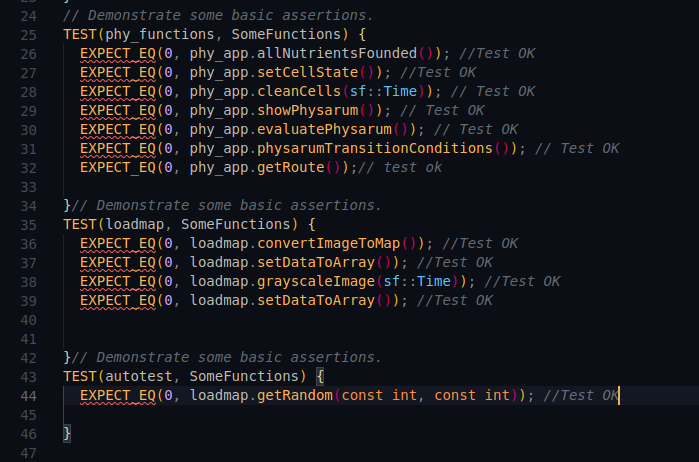
\includegraphics[width=0.5\textwidth]{./images/Pruebas/simulador/image041.png}
        \caption{Prueba unitaria 1}
        \label{fig:Prueba unitaria 1}
    \end{figure}
    Las funciones mostradas son las que fueron agregadas al
        archivo de pruebas unitarias que ya se hab\'ian realizado junto
        con las nuevas aplicadas debido a la introducci\'on de nuevas
        funcionalidades dentro del programa. Como podemos ver,
        todas las pruebas resultaron exitosas, lo que es esperable al
        menos en su mayor\'ia, ya que como se mencion\'oanteriormente en las primeras pruebas unitarias, el programa
        funciona a partir de un modelo matem\'atico y debido a su
        naturaleza, el funcionamiento depende de que la
        implementaci\'on de ese modelo matem\'atico a trav\'es del
        algoritmo sea correcta.
        \vskip 0.5cm
    Las nuevas funciones corresponden a la implementaci\'on de
        la lectura de im\'agenes a transformar en mapas al inicio del
        programa, lo que facilita la entrada de entornos en los cuales
        se quiera simular al Physarum.
        \vskip 0.5cm